\documentclass[9pt, aspectratio=169, handout]{beamer}

% +==================================================+
% |   ████████╗██╗  ██╗███████╗███╗   ███╗███████╗   |
% |   ╚══██╔══╝██║  ██║██╔════╝████╗ ████║██╔════╝   |
% |      ██║   ███████║█████╗  ██╔████╔██║█████╗     |
% |      ██║   ██╔══██║██╔══╝  ██║╚██╔╝██║██╔══╝     |
% |      ██║   ██║  ██║███████╗██║ ╚═╝ ██║███████╗   |
% |      ╚═╝   ╚═╝  ╚═╝╚══════╝╚═╝     ╚═╝╚══════╝   |
% +==================================================+

\useinnertheme{rectangles}
\useoutertheme{infolines}

\setbeamertemplate{footline}{%
    \leavevmode%
    \rule{\paperwidth}{0.1pt}\vskip0.2pt%
    \hbox{%
        \begin{beamercolorbox}[wd=.2\paperwidth, ht=2.25ex, dp=1ex, center]{author in head/foot}%
            \usebeamerfont{author in head/foot}\insertshortauthor
        \end{beamercolorbox}%
        \begin{beamercolorbox}[wd=.6\paperwidth, ht=2.25ex, dp=1ex, center]{title in head/foot}%
            \usebeamerfont{title in head/foot}\insertshorttitle
        \end{beamercolorbox}%
        \begin{beamercolorbox}[wd=.2\paperwidth, ht=2.25ex, dp=1ex, center]{date in head/foot}%
            \usebeamerfont{date in head/foot}\insertshortdate\hfill\insertframenumber{} / \inserttotalframenumber\hspace*{2ex}
        \end{beamercolorbox}%
    }%
    \vskip0pt%
}
% hrule under the frametitle, see:
% https://tex.stackexchange.com/questions/343517/beamer-full-width-hrule-below-frame-title
\setbeamertemplate{frametitle}{%
    \usebeamerfont{frametitle}\insertframetitle%
    \vphantom{g}%
    \par%
    \makebox[\linewidth][c]{%
        \rule[0.5\baselineskip]{\paperwidth}{0.4pt}%
    }%
}

% \beamertemplatenavigationsymbolsempty % remove navigation bar

\definecolor{grey80}{HTML}{CCCCCC}
\definecolor{grey90}{HTML}{E6E6E6}
\definecolor{grey95}{HTML}{F2F2F2}

\usepackage[svgnames, x11names]{xcolor}
\usecolortheme[named=DarkSlateGrey]{structure}
\setbeamercolor{background canvas}{bg=white}

\setbeamerfont{frametitle}{series=\bfseries}

\let\oldtiny\tiny
\let\oldscriptsize\scriptsize
\let\oldfootnotesize\footnotesize
\let\oldsmall\small
\let\oldnormalsize\normalsize
\let\oldlarge\large
\let\oldLarge\Large
\let\oldLARGE\LARGE
\let\oldhuge\huge
\let\oldHuge\Huge
\renewcommand*{\footnotesize}{\oldfootnotesize\scriptsize}
\renewcommand*{\normalsize}{\oldnormalsize\oldsmall}
\setbeamerfont{frametitle}{size=\oldnormalsize}

% +=================================+
% |   ██████╗ ██╗██████╗ ███████╗   |
% |   ██╔══██╗██║██╔══██╗██╔════╝   |
% |   ██████╔╝██║██████╔╝███████╗   |
% |   ██╔══██╗██║██╔══██╗╚════██║   |
% |   ██████╔╝██║██████╔╝███████║   |
% |   ╚═════╝ ╚═╝╚═════╝ ╚══════╝   |
% +=================================+

% \usepackage[style=nejm,backend=biber]{biblatex}
% \addbibresource{my.bib}
% \renewcommand*{\bibfont}{\footnotesize}

% +==========================================+
% |   ███╗   ███╗ █████╗ ████████╗██╗  ██╗   |
% |   ████╗ ████║██╔══██╗╚══██╔══╝██║  ██║   |
% |   ██╔████╔██║███████║   ██║   ███████║   |
% |   ██║╚██╔╝██║██╔══██║   ██║   ██╔══██║   |
% |   ██║ ╚═╝ ██║██║  ██║   ██║   ██║  ██║   |
% |   ╚═╝     ╚═╝╚═╝  ╚═╝   ╚═╝   ╚═╝  ╚═╝   |
% +==========================================+

\usepackage{amsmath,amssymb,amsfonts}
\usepackage{cancel}
\usepackage{braket}
\usepackage{bm}
\usepackage{siunitx}
\usepackage{feynmf}
\usepackage{cleveref}
\DeclareGraphicsRule{*}{mps}{*}{}

% +===================================================+
% |   ███████╗██╗ ██████╗ ██╗   ██╗██████╗ ███████╗   |
% |   ██╔════╝██║██╔════╝ ██║   ██║██╔══██╗██╔════╝   |
% |   █████╗  ██║██║  ███╗██║   ██║██████╔╝█████╗     |
% |   ██╔══╝  ██║██║   ██║██║   ██║██╔══██╗██╔══╝     |
% |   ██║     ██║╚██████╔╝╚██████╔╝██║  ██║███████╗   |
% |   ╚═╝     ╚═╝ ╚═════╝  ╚═════╝ ╚═╝  ╚═╝╚══════╝   |
% +===================================================+
\usepackage{subcaption}
\usepackage{makecell}
\usepackage{booktabs}

% +===========================================================+
% |    ██████╗██╗  ██╗██╗███╗   ██╗███████╗███████╗███████╗   |
% |   ██╔════╝██║  ██║██║████╗  ██║██╔════╝██╔════╝██╔════╝   |
% |   ██║     ███████║██║██╔██╗ ██║█████╗  ███████╗█████╗     |
% |   ██║     ██╔══██║██║██║╚██╗██║██╔══╝  ╚════██║██╔══╝     |
% |   ╚██████╗██║  ██║██║██║ ╚████║███████╗███████║███████╗   |
% |    ╚═════╝╚═╝  ╚═╝╚═╝╚═╝  ╚═══╝╚══════╝╚══════╝╚══════╝   |
% +===========================================================+

% \usepackage{xeCJK}
% \setCJKmainfont{PingFang SC}

% +====================================+
% |   ███╗   ███╗██╗███████╗ ██████╗   |
% |   ████╗ ████║██║██╔════╝██╔════╝   |
% |   ██╔████╔██║██║███████╗██║        |
% |   ██║╚██╔╝██║██║╚════██║██║        |
% |   ██║ ╚═╝ ██║██║███████║╚██████╗   |
% |   ╚═╝     ╚═╝╚═╝╚══════╝ ╚═════╝   |
% +====================================+

\usepackage{fontawesome5}
\usepackage{twemojis}
\newcommand{\myhl}[1]{\textcolor{DeepPink}{#1}}
\newcommand{\myhlb}[1]{\textcolor{Blue}{#1}}


\title{MAE 131A Discussion Sections\\ Week 4}
\author{Chuanjin Su}
\institute[UCLA MAE]{Mechanical and Aerospace Engineering Department\\
    University of California, Los Angeles}
\date{Oct 25, 2024}

\begin{document}

\begin{frame}
    \titlepage
\end{frame}

\begin{frame}{Problem 1 (6.44 in \textit{AHTT})}
    For uniform wall heat flux $q_w$, Churchill and Ozoe proposed the following correlation with $\mathrm{Pe}_x > 100, q_w = \text{constant}$ over the full range of $\mathrm{Pr}$:
    \begin{equation}
        \mathrm{Nu}_x = \frac{0.464\mathrm{Re}_x^{1/2}\mathrm{Pr}^{1/3}}{\Big[1 + (0.0205 / \mathrm{Pr})^{2/3}\Big]^{1/4}}
        \tag{6.73 in \textit{AHTT}}
    \end{equation}
    \textbf{Problem 6.44}. Beginning with eqn. (6.73), show that $\overline{\mathrm{Nu}}_L$ is given over the entier range of $\mathrm{Pr}$ for a laminar b.l. on a flat, constant flux surface by:
    \begin{equation}
        \overline{\mathrm{Nu}}_L = \frac{0.696\overline{\mathrm{Re}}_L^{1/2}\mathrm{Pr}^{1/3}}{\Big[1 + (0.0205 / \mathrm{Pr})^{2/3}\Big]^{1/4}}
    \end{equation}
\end{frame}

\begin{frame}{Porblem 1 Solution}
    \textbf{Solution}. For averaging the Nusselt number for the constant heat flux, an \myhl{average temperature difference} must be the reference to calculate the average heat transfer coefficient. Since $\mathrm{Nu}_x\propto x^{1/2}$ and $\mathrm{Nu}_x = \frac{h(x)x}{k}$, thus $h(x)\propto x^{-1/2}$, resulting in $(T-T_{\infty})\propto x^{1/2}$. Therefore, $\overline{T_w - T_{\infty}} = \frac{1}{L}\int_0^L (T_w - T_{\infty}) \mathrm{d}x \propto \frac{2}{3}L^{1/2}$. The average Nusselt number is then proportional to $\frac{3}{2}L^{1/2}$ due to $\overline{\mathrm{Nu}}_L = \frac{q_w L}{k(\overline{T_w - T_{\infty}})}$. Absorbing the proportionality, we have,
    \begin{equation}
        \overline{\mathrm{Nu}}_L = \frac{0.696\overline{\mathrm{Re}}_L^{1/2}\mathrm{Pr}^{1/3}}{\Big[1 + (0.0205 / \mathrm{Pr})^{2/3}\Big]^{1/4}}
    \end{equation}
    \hfill\qedsymbol

    \textbf{Comment}. The key point for this problem is that,
    \begin{equation}
        \overline{h} \neq \frac{1}{L}\int_0^L h(x) \mathrm{d}x.
    \end{equation}
    Instead, the Newton's law of cooling must hold after averaging, i.e.,
    \begin{equation}
        \overline{h} \cdot \overline{T_w - T_{\infty}} = \overline{q_w}, \qquad\Rightarrow \overline{h} = \frac{\overline{q_w}}{\overline{T_w - T_{\infty}}}.
    \end{equation}
\end{frame}

\begin{frame}{Problem 2 (7.36 in the book)}
    \textbf{Problem 7.36}. Air at \SI{27}{\degree C} with a free stream velocity of \SI{10}{m/s} is used to cool electronic devices mounted on a printed circuit board. Each device, \SI{4}{mm} $\times$ \SI{4}{mm}, dissipates \SI{40}{mW}, which is removed from the top surface. A turbulator is located at the leading edge of the board, causing the boundary layer to be turbulent. Estimate the surface temperature of the fourth device located \SI{15}{mm} from the leading edge of the board.
    \begin{figure}
        \begin{center}
            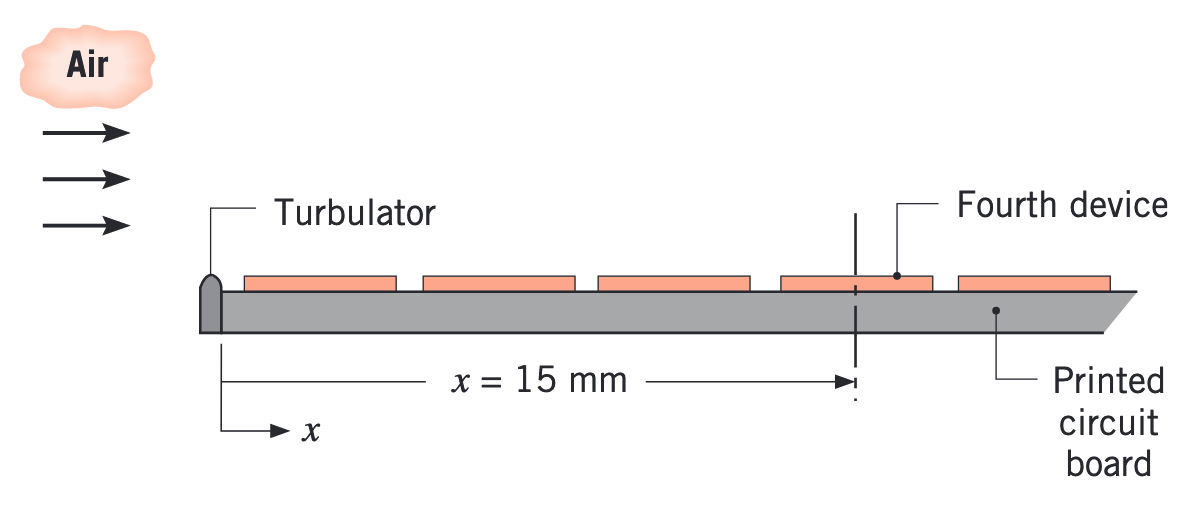
\includegraphics[width=0.4\textwidth]{Figures/fig4.1.png}
        \end{center}
    \end{figure}
    \textbf{Hint}. Use the following properties: Air (assume $\mathrm{T}_s=\SI{330}{K}$, thus $\bar{T} = \SI{315}{K}$, \SI{1}{atm}): $k = \SI{0.0274}{W/m.K}, \nu=\SI{17.40e-6}{m^2/s}, \alpha=\SI{24.7e-6}{m^2/s}, \mathrm{Pr} = 0.705$. The turbulent correlation is $\mathrm{Nu}_x = 0.0296\mathrm{Re}_x^{4/5}\mathrm{Pr}^{1/3}$ (eqn. 6.112 in \textit{AHTT}).
\end{frame}

\begin{frame}{Problem 2 Solution}
    \textbf{Solution}. Since flow is turbulent, it is reasonable to assume that thermal properties for the whole surface of the fourth device are all uniform.
    \begin{equation}
        \mathrm{Re}_x = \frac{u_\infty x}{\nu} = \frac{10\times 0.015}{17.40\times 10^{-6}} = 8.6207\times 10^3
    \end{equation}
    giving
    \begin{equation}
        \mathrm{Nu}_x = 0.0296 \times (8.6207\times 10^3)^0.8 \times 0.705^{1/3} = 37.08 = \frac{h(x) x}{k}
    \end{equation}
    thus $h(x) = \mathrm{Nu}_x k / x = \SI{67.73}{W/m^2.K}$. Therefore, the surface temperature is,
    \begin{equation}
        T_s = \SI{300}{K} + \frac{\SI{40e-3}{W}}{\SI{67.73}{W/m^2.K}\times (\SI{4e-3}{m})^2} = \SI{336.9}{K}.
    \end{equation}
    \hfill\qedsymbol
\end{frame}

\begin{frame}{Problem 3 (7.45 in the book)}
    \begin{columns}
        \column{0.8\textwidth}
        \textbf{Problem 7.45}. A square ($\SI{10}{mm}\times \SI{10}{mm}$) silicon chip is insulated on one side and cooled on the opposite side by atmospheric air in parallel flow at $u_{\infty}=\SI{20}{m/s}$ and $T_{\infty} = \SI{24}{\degree C}$.
        When in use, electrical power dissipation within the chip maintains a uniform heat flux at the cooled surface. If the chip temperature may not exceed \SI{80}{\degree C} \myhl{at any point on its surface}, what is the maximum allowable power?

        \vspace{1em}

        \textbf{Hint}. For laminar flow over a flat plate with constant heat flux, the Nusselt number is given by,
        \begin{equation*}
            \begin{aligned}
                \mathrm{Nu}_x &= 0.453\mathrm{Re}_x^{1/2}\mathrm{Pr}^{1/3}, \quad \mathrm{Pr} \gtrsim 0.6 \\
                \overline{\mathrm{Nu}}_L &= 0.680\overline{\mathrm{Re}}_L^{1/2}\mathrm{Pr}^{1/3}.
            \end{aligned}
        \end{equation*}
        Use the following properties for air: $\nu = \SI{18.41e-6}{m^2/s}, k = \SI{0.0282}{W/m.K}, \mathrm{Pr} = 0.703$.
        
        Ignore the heat conduction inside the chip.
    \end{columns}
\end{frame}

\begin{frame}{Problem 3 Solution}
    \textbf{Solution}. The Reynolds number is $1.09 \times 10^4$, resulting in laminar flow. Since the temperature varies with $x$, we have to consider the maximum temperature on the surface, which should be at the trailing edge where the heat transfer coefficient is the lowest.
    \begin{equation*}
        h_L = \frac{k}{L} \times 0.453 \mathrm{Re}_L^{1/2} \mathrm{Pr}^{1/3} = \SI{118}{W/m^2.K},
    \end{equation*}
    the maximum allowable heat flux is thus,
    \begin{equation*}
        q''_{\text{max}} = h_L (T_{\text{max}} - T_{\infty}) = \SI{118}{W/m^2.K} \times (80 - 24) \si{\degree C} = \SI{6630}{W/m^2},
    \end{equation*}
    and the total power is $q_{\text{max}} = q''_{\text{max}} \times (\SI{1e-2}{m})^2 = \SI{0.66}{W}$. \hfill\qedsymbol
\end{frame}

\end{document}
